\documentclass{article}

% Recommended, but optional, packages for figures and better typesetting:
\usepackage{microtype}
\usepackage{graphicx}
\usepackage{subfigure}
\usepackage{booktabs} % for professional tables

\usepackage{tikz}
% Corporate Design of the University of Tübingen
% Primary Colors
\definecolor{TUred}{RGB}{165,30,55}
\definecolor{TUgold}{RGB}{180,160,105}
\definecolor{TUdark}{RGB}{50,65,75}
\definecolor{TUgray}{RGB}{175,179,183}

% Secondary Colors
\definecolor{TUdarkblue}{RGB}{65,90,140}
\definecolor{TUblue}{RGB}{0,105,170}
\definecolor{TUlightblue}{RGB}{80,170,200}
\definecolor{TUlightgreen}{RGB}{130,185,160}
\definecolor{TUgreen}{RGB}{125,165,75}
\definecolor{TUdarkgreen}{RGB}{50,110,30}
\definecolor{TUocre}{RGB}{200,80,60}
\definecolor{TUviolet}{RGB}{175,110,150}
\definecolor{TUmauve}{RGB}{180,160,150}
\definecolor{TUbeige}{RGB}{215,180,105}
\definecolor{TUorange}{RGB}{210,150,0}
\definecolor{TUbrown}{RGB}{145,105,70}

% hyperref makes hyperlinks in the resulting PDF.
% If your build breaks (sometimes temporarily if a hyperlink spans a page)
% please comment out the following usepackage line and replace
% \usepackage{icml2023} with \usepackage[nohyperref]{icml2023} above.
\usepackage{hyperref}


% Attempt to make hyperref and algorithmic work together better:
\newcommand{\theHalgorithm}{\arabic{algorithm}}

\usepackage[accepted]{icml2023}

% For theorems and such
\usepackage{amsmath}
\usepackage{amssymb}
\usepackage{mathtools}
\usepackage{amsthm}

% if you use cleveref..
\usepackage[capitalize,noabbrev]{cleveref}

%%%%%%%%%%%%%%%%%%%%%%%%%%%%%%%%
% THEOREMS
%%%%%%%%%%%%%%%%%%%%%%%%%%%%%%%%
\theoremstyle{plain}
\newtheorem{theorem}{Theorem}[section]
\newtheorem{proposition}[theorem]{Proposition}
\newtheorem{lemma}[theorem]{Lemma}
\newtheorem{corollary}[theorem]{Corollary}
\theoremstyle{definition}
\newtheorem{definition}[theorem]{Definition}
\newtheorem{assumption}[theorem]{Assumption}
\theoremstyle{remark}
\newtheorem{remark}[theorem]{Remark}

% Todonotes is useful during development; simply uncomment the next line
%    and comment out the line below the next line to turn off comments
%\usepackage[disable,textsize=tiny]{todonotes}
\usepackage[textsize=tiny]{todonotes}
\usepackage{float}

% The \icmltitle you define below is probably too long as a header.
% Therefore, a short form for the running title is supplied here:
\icmltitlerunning{Comparing different active learning query methods}

\begin{document}

\twocolumn[
\icmltitle{Active Learning: Because Guesswork is Overrated}

% It is OKAY to include author information, even for blind
% submissions: the style file will automatically remove it for you
% unless you've provided the [accepted] option to the icml2023
% package.

% List of affiliations: The first argument should be a (short)
% identifier you will use later to specify author affiliations
% Academic affiliations should list Department, University, City, Region, Country
% Industry affiliations should list Company, City, Region, Country

% You can specify symbols, otherwise they are numbered in order.
% Ideally, you should not use this facility. Affiliations will be numbered
% in order of appearance and this is the preferred way.
\icmlsetsymbol{equal}{*}

\begin{icmlauthorlist}
	\icmlauthor{Lukas Weber, lukas.weber@studenti.unitn.it}{first}
\end{icmlauthorlist}

\icmlaffiliation{first}{MSc Computer Science, Tübingen, GER}
\icmlcorrespondingauthor{Lukas Weber}{lukas2.weber@student.uni-tuebingen.de}


% You may provide any keywords that you
% find helpful for describing your paper; these are used to populate
% the "keywords" metadata in the PDF but will not be shown in the document
\icmlkeywords{Machine Learning, Active Learning}

\vskip 0.3in
]

% this must go after the closing bracket ] following \twocolumn[ ...

% This command actually creates the footnote in the first column
% listing the affiliations and the copyright notice.
% The command takes one argument, which is text to display at the start of the footnote.
% The \icmlEqualContribution command is standard text for equal contribution.
% Remove it (just {}) if you do not need this facility.

%\printAffiliationsAndNotice{}  % leave blank if no need to mention equal contribution
%\printAffiliationsAndNotice{\icmlEqualContribution} % otherwise use the standard text.

\begin{abstract}
	A huge amount of unlabeled data is typically available but annotating large datasets is often costly and time-consuming, making active learning a crucial tool for selecting the most informative samples to minimize annotation efforts. This report compares different active learning query strategies using the modAL framework in a pool-based setting. In experiments, a logistic regression model and an ensemble of such models is evaluated on the MNIST dataset. The impact of different query strategies is analyzed, including Uncertainty Sampling, Margin Sampling, Entropy Sampling (including ensemble adaptions) and Ranked batch-mode Sampling. Findings indicate that querying samples with Margin Sampling achieves the highest accuracy and fastest convergence. While ensemble models show faster convergence with small datasets, they provide shrinking improvements over single models as dataset size increases. These results highlight the high importance of query strategy selection on model performance in active learning pipelines and explore conditions under which ensemble models may improve performance.
\end{abstract}


\section{Introduction and Related Work}\label{sec:intro}
Supervised learning often requires large, annotated datasets. However obtaining high-quality labeled data can be costly and time-intensive, especially expert knowledge is required, such as medical imaging. Though, unlabeled data is usually easily available. 
Active learning addresses this challenge by reducing the overall labeling costs through the selection of most informative samples for annotation based on a query strategy. This approach enables machine learning models to perform well in tasks with limited data and high labeling costs. \\
The effectiveness of active learning is tied to the chosen query strategy, that determines which unlabeled samples are selected for annotation and then added to the training set. \\
This report evaluates several strategies in a pool-based active learning setting: A model is initially trained on a small labeled dataset and used to evaluate a large pool of unlabeled data. The most informative samples are selected based on a query strategy, they are then labeled by an oracle, and added to the training set. The model is retrained with the updated training set and the process is repeated until a stopping criterion is met.
Experiments in this paper leverage the modular Active Learning framework (modAL)~\cite{danka_modalmodularactivelearning}, which simplifies the implementation of active learning pipelines, includes multiple pre-implemented query strategies and is compatible with Scikit-learn models~\cite{scikit-learn}. \\
The experiments focus on the image domain, using the MNIST dataset~\cite{mnist}, and examine the impact of query strategies on a single logistic regression model and a committee-based approach.
Several previous works have explored and compared different query methods across various domains. \cite{schröder_revisitinguncertaintybasedquerystrategies} compared various uncertainty-based query strategies in the context of fine-tuning transformer models in text classification tasks, while \cite{zhan_comparativesurveydeepactive} examined several query methods in image classification tasks using MNIST and CIFAR. \\
According to \cite{ueno_benchmarkingofquerystrategies} most papers concentrate on two image-based datasets: MNIST~\cite{mnist} and CIFAR~\cite{cifar}, while their paper evaluates strategies on six different datasets, including medical and visual inspection images. They also examine strategies independent of training processes to minimize biases from early-stage randomness or underfitting. This is shown in an experiment where fully trained models are used to select the most informative samples based on several different query strategies to construct a labeled dataset. \\ 
A recurring issue in active learning research is the lack of standardization in experimental setups, making it difficult to compare existing and new query strategies, as noticed additionally by~\cite{werner_comparableactivelearning}. This inconsistency complicates the comparability of existing and novel query strategies. To address this, they propose a benchmark framework for evaluating active learning strategies across tabular, image and text datasets. This framework uses robust evaluation protocols to reduce variance and ensure comparability. \\
In contrast, \cite{ueno_benchmarkingofquerystrategies} focus specifically on image-based datasets from diverse domains such as medical or visual inspection images. While~\cite{werner_comparableactivelearning} focuses on a wide range of data-domains including images, text and vector-based datasets.
This work focuses on query strategy comparisons within the image domain, specifically for a logistic regression model and an ensemble-based approach on MNIST. \\
The contributions of this paper are as follows:
\begin{itemize}
	\item A systematic evaluation of active learning query strategies using \textbf{logistic regression on MNIST}.
	\item \textbf{Investigation of the incluence of model aggregation} on the effectiveness of query strategies to provide insights into how these models respond differently to active learning methods.
\end{itemize}
Section~\ref{sec:methods} outlines the used dataset, processing steps and models and describes the experimental design, followed by the results and discussion in sections~\ref{sec:results} and~\ref{sec:discussion} respectively. The report concludes with key findings in section~\ref{sec:conclusion}. \\
\\
The corresponding implementation can be found on \textcolor{red}{\href{https://github.com/LukaslWeber/NLP_II_Interactive_Learning}{Github}}.

\section{Methods}\label{sec:methods}
The following section describes the dataset which was used in experiments, preprocessing steps, the logistic regression model and other parameters which are needed for reproducibility.
\subsection{Dataset}
MNIST is a dataset consisting of handwritten digits with 60.000 train samples and 10.000 test samples. Digits are size-normalized and centered in a $28 \times 28$ image~\cite{mnist}. Each digit belongs to one of 10 classes, corresponding to the  numbers from 0 to 9. \\
Upon loading the dataset, each image is vectorized, i.e. transformed from a $28 \times 28$ sized image-matrix to a vector of length $784$. Furthermore, each pixel initially contains a grayscale value ranging from 0 to 255. Pixel values are additionally normalized to a range between 0 and 1 in order to provide a value range that works well with logistic regression.
%\\
%\\
%CIFAR-10 is a dataset which consists of 50.000 train- and 10.000 test-images. Each natural image belongs to one of 10 classes. Each class has exactly 5.000 train and 1.000 test images. The image-size is $32 \times 32$ pixels. 
%\textcolor{red}{CIFAR preprocessing split}. CIFAR-10 includes real-world images and is thus expected to be more complicated to learn.
%
MNIST is a class-balanced dataset, i.e. each class has roughly the same number of samples as any other class.

\subsection{Multinomial Logistic Regression Model}
Sklearn's LogisticRegression module is used to predict digits with the given data from MNIST. Multinomial logistic regression predicts a probability for each possible class instead of a single probability as in Binomial logistic regression.
\\
The model estimates the probability $P(y=i \mid X)$ of a sample belonging to class $i$ using the SoftMax function:
\begin{align}
	P(y=i \mid X)=\frac{\exp \left(X \beta_i\right)}{\sum_{j=1}^k \exp \left(X \beta_j\right)}
\end{align}
where $\beta_i$ are the coefficients for class $i$. The SoftMax function ensures that probabilities across classes sum to 1 and consequently that a model creates a probability distribution over the classes. \\
During training, the model maximizes the likelihood of the observed data:
\begin{align}
	\mathcal{L}(\beta)=\prod_{n=1}^N \prod_{i=1}^k\left(P\left(y_n=i \mid X_n\right)\right)^{y_{n i}}
\end{align}
where $N$ is the number of samples, and $y_{n i}$ indicates if sample $n$ belongs to class $i$. $k=10$ denotes the number of classes. \\
The likelihood of the observed data is maximized by minimizing the Cross-Entropy loss $\mathcal{L}$ which is defined as:
\begin{align}
	\mathcal{L}=-\frac{1}{N} \sum_{n=1}^N \sum_{j=1}^k y_{n j} \log \left[P\left(y=j \mid X_n\right)\right]
\end{align}
To find hyperparameters which maximize performance on the given dataset, 5-fold-cross-validation is used with a grid-search, testing out a variety solvers, regularization methods and corresponding strengths, maximum iterations and stopping-tolerance options. \\
The resulting models use the "newton-cg" solver which combines Newton's method with conjugate gradient descent. It uses the gradient and the second order derivative of $\mathcal{L}$ given by the Hessian matrix to iteratively find the minimum of $\mathcal{L}$. \\
Regularization using the $\ell_2$-norm prevents overfitting with a strength $C=0.01$ in addition to a stopping-criterion $tol=0.0001$, which stops the learning process when the $\ell_2$-norm of the gradient of $\mathcal{L}$ is lower than $tol$, indicating convergence. \\
For reproducibility purposes, the same random seed ($42$) is used to initialize all random number generators and single model weights. Weights of models in an ensemble are initialized with a fixed set of random seeds (42, 43, 44, 45, 46) to introduce diversity. These measures ensure that same configurations lead to the same outcomes, even when training models in succession. 

\subsection{Active Learning}
In the following experiments, a single logistic regression model is compared to a committee of 5 models across different query strategies. The committee predicts by averaging the class probabilities obtained by each learner, called the consensus probabilities. The final prediction is the class with the highest consensus probability. \\
In pool-based active learning, an initial labeled dataset is required. When a single model is used for training and querying new samples, $n_{init}=75$ labeled instances are used to train the model initially, ensuring a moderate fit before querying samples. This is done to make sure that initial samples are chosen on a meaningful basis and do not bias the rest of the training negatively. For the committee, each model is initialized with $60\%$ randomly chosen samples from the initial labeled train set, resulting in $45$ initial data points per model. \\
For both methods, models are trained for $init\_max\_iter=50$ epochs on the initial dataset. $init\_max\_iter$ is based on the hyperparameters found by 5-fold-cross-validation and ensures a sufficient fit to the datapoints. Thus, reducing the bias from early queried samples which were chosen when model predictions are inaccurate. \\
After initial training, 5 samples are queried at a time for 1000 iterations, resulting in 5000 additional samples at the end of the learning process. After quering, the new samples are added to the training set and models are fine-tuned for $n_{iter}=20$ iterations. 
\subsection{Query Strategies}
A multitude of query strategies are used to compare a single model to an ensemble of models. As a control metric, Random Sampling is used to give a baseline for other query strategies.\\
Uncertainty Sampling selects the least certain instances for labeling.
\begin{align}
	Uncertainty(\mathbf{x})=1-P_\theta(\hat{y} \mid \mathbf{x})
\end{align}
Where $\hat{y}=\operatorname{arg}\underset{y}{\operatorname{max}} \ p_\theta(y \mid \mathbf{x})$, i.e. corresponds to the predicted class of the model and $P_\theta$ is the probability to predict class $\hat{y}$ with the model with parameters $\theta$. \\
Entropy Sampling selects instances with the highest entropy to query for labeling, focusing on the most ambiguous cases. It measures the amount of information needed to encode a distribution and is often used as a measure of uncertainty.
\begin{align}
	\mathcal{H}(\mathbf{x})=-\sum_{i=0}^{9} P_\theta(y_i \mid \mathbf{x}) \log P_\theta(y_i \mid \mathbf{x})
\end{align}
Where $y_i$ stands for the probability to predict class $i$. \\
Vote Entropy Sampling is a query strategy designed for ensemble models. It calculates the ensemble predictions, then calculates the probability distribution over the predictions which are used to determine the Entropy $\mathcal{H}$. Vote Entropy then selects instances with the highest Entropy. \\
Margin Sampling selects the instances where the difference between the most likely and second most likely class is the smallest, indicating high ambiguity.
\begin{align}
	Margin(\mathbf{x})=P_\theta\left(\hat{y}_1 \mid \mathbf{x}\right)-P_\theta\left(\hat{y}_2 \mid \mathbf{x}\right)
\end{align}
where $\hat{y}_1$ and $\hat{y}_2$ are the most likely and the second likely predicted labels given by $\hat{y}_1=\operatorname{arg}\underset{y}{\operatorname{max}} \  p_\theta(y \mid x)$ and $\hat{y}_2=\operatorname{arg}\underset{y \neq \hat{y}_1}{\operatorname{max}} \  p_\theta(y \mid x)$, respectively. \\
Ranked batch-mode Sampling~\cite{ranked_batch_mode_query_strategy} weights uncertainty and diversity. It is designed for querying multiple samples, as traditional approaches such as uncertainty sampling may add redundant samples when querying multiple samples at once. \\
\begin{align}
	RBM(x)&=\alpha \left(1-\Phi\left(x, X_{\text {labeled }}\right)\right) \notag \\ &+(1-\alpha) \ Uncertainty(x)
\end{align}
Where $\alpha=\frac{\left|X_{\text {unlabeled}}\right|}{\left|X_{\text {unlabeled}}\right|+\left|X_{\text {labeled}}\right|}$, $X_{\text {labeled}}$ and $X_{\text {unlabeled}}$ are the labeled dataset and unlabeled pool, respectively. $\Phi$ denotes the similarity given by the Cosine Similarity metric.
\begin{figure*}[!h]
	\begin{center}
		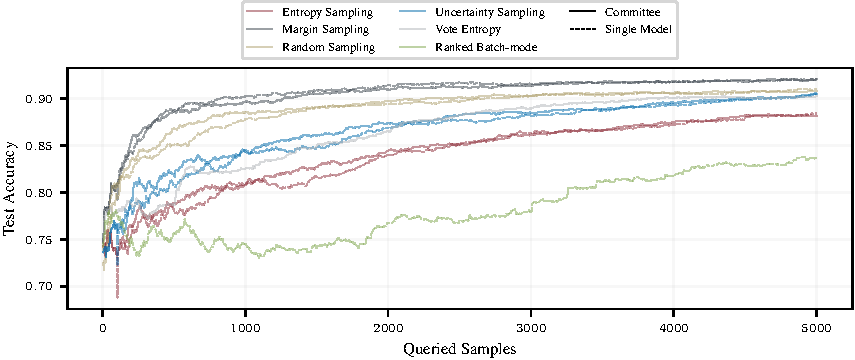
\includegraphics[width=0.95\linewidth]{fig/test_accuracy.pdf}
	\end{center}
	\caption{Test accuracy versus the number of annotated samples that were added to the train dataset by querying instances. As examples are queried and added to the training dataset, the model is retrained, and its performance is evaluated on the test set.}
	\label{accuracy_plot}
\end{figure*}
\begin{figure*}[!h]
	\begin{center}
		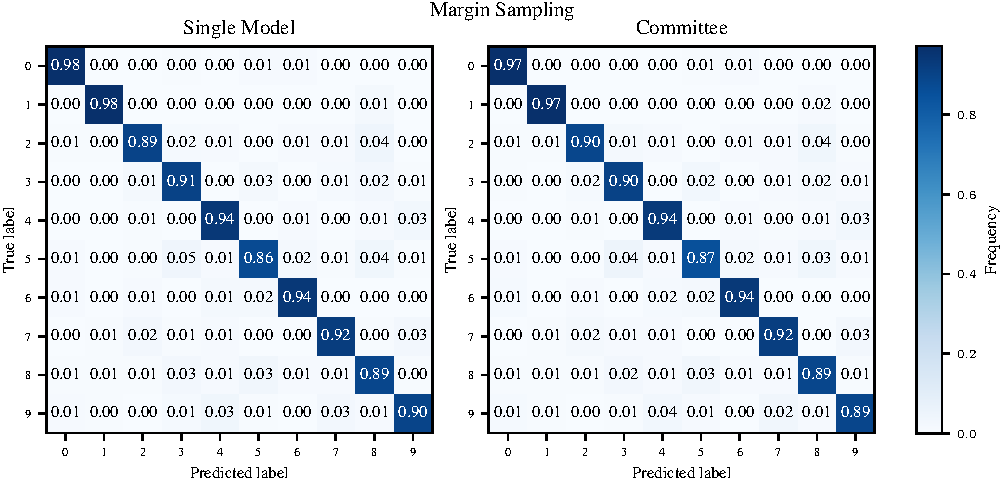
\includegraphics[width=0.95\linewidth]{fig/conf_mat_margin_sampling.pdf}
	\end{center}
	\caption{Confusion Matrix of models trained with Margin Sampling.}
	\label{conf_mat_margin_sampling}
\end{figure*}
\subsection{Evaluation metrics}
In the following section, multiple evaluation metrics are used to gain insights into understanding the differences and quality of each query method and the single-model vs. ensemble-model approach. \\
Due to the fact, that MNIST is class-balanced, a well-working metric is the accuracy. It is defined as as the number of correctly classified instances divided by the total number of instances. \\
Furthermore, confusion matrices are created to evaluate systemic errors in the prediction of certain numbers.  
\section{Results}\label{sec:results}
A Logistic Regression model that is trained on the whole labeled train dataset of MNIST reaches a test accuracy of $92.58\%$. This serves as a theoretical maximum that can be reached given a sufficient amount of train data. \\
By plotting the accuracy on the test samples vs. the number of queried examples in figure~\ref{accuracy_plot}, convergence behaviour of different query methods can be analyzed. On MNIST, Margin Sampling reaches the highest Accuracy with 92.08\% for both models and converges the fastest, followed by Random Sampling. Entropy Sampling and Uncertainty Sampling perform worse than Random Sampling. Only after querying 5000 additional samples, the difference in accuracy between both strategies and Random Sampling is 0.25\%. For most query strategies, performance between a single model and an ensemble of models does not differ. \\
Furthermore, it can be seen that ensemble models converge faster than single models with the same query method, with small train datasets, but differences between models shrink with an increased number of queried samples. \\
The ensemble that is trained with Vote Entropy sampling performs better than the models trained with Entropy sampling with an accuracy difference of 2.08\% to the single model and 1.79\% to the ensemble, indicating that query strategies specifically adapted for ensemble models can boost classification performance. \\
Figure~\ref{conf_mat_margin_sampling} and shows the confusion matrices of the best performing query strategy, Margin Sampling. The single model trained with Margin Sampling achieves the lowest accuracy of $86\%$ when an input image contains the number 5, whereas the ensemble reaches has 1\% more accuracy in this case, which also resembles the worst number for the ensemble. In both cases, the most likely prediction is 3 when the number 5 is shown. 

\section{Discussion}\label{sec:discussion}
Results show that Margin Sampling achieves the highest accuracy and fastest convergence by prioritizing instances with the greatest ambiguity, effectively adding diversity to the training dataset. It does not show high systemic errors. In contrast, Uncertainty and Entropy Sampling underperform compared to Random Sampling, possibly due to redundant sample selection. \\
Across query strategies, the ensemble converges faster than single models the smaller train datasets are, leveraging prediction diversity in early stages. However, its advantage diminishes as the labeled train dataset grows. This leads to the conclusion that ensembles help to reduce the impact of single model biases in small datasets. For most strategies, the ensemble's added diversity does not translate into substantial performance gains, as shown by its marginal improvement over single models. Both, single and ensemble models, converge similarly for the same sampling strategy, indicating that a single Logistic Regression Model is able to effectively learn MNIST when given enough data. Furthermore, early biases can be reduced by using an ensemble. Using more complex models and data might lead to the ensemble converging to a higher accuracy than single models, as is often seen. \\
This study uses a logistic regression model and a simple, balanced dataset, which simplifies the analysis but limits generalizability. While the findings highlight the effectiveness of certain strategies for shallow models, it is unclear if these results hold for more complex models or imbalanced datasets.
Future work should explore diverse data types, like text, tabular or time series data, complex models, and imbalanced datasets to better understand the broader applicability of these findings and see whether complex models show similar convergence profiles.


\section{Conclusion}\label{sec:conclusion}
This report systematically evaluated active learning query strategies using logistic regression on MNIST. Margin Sampling is shown to be the most effective strategy, achieving the highest accuracy and fastest convergence by focusing on instances with the greatest ambiguity. Ensemble models demonstrated faster convergence in early training stages, possibly due to higher diversity but offered limited performance gains over single models as labeled datasets grew. \\
Key findings suggest that ensembles are particularly advantageous when dealing with small datasets, reducing biases from single-model predictions. However, since single logistic regression models already perform well on MNIST when there’s enough labeled data, using an ensemble doesn’t add much benefit in this case. The underperformance of uncertainty- and entropy-based strategies compared to Random Sampling indicates that redundant sample selection remains a challenge, as Random Sampling may unintentionally add variety to the data. \\
Future research should extend these insights to more complex models and datasets, including imbalanced and multi-domain scenarios such as text and tabular data. Additionally, exploring novel query strategies tailored to diverse use cases could further optimize active learning pipelines for real-world applications.

\bibliography{bibliography}
\bibliographystyle{icml2023}

\end{document}


% This document was modified from the file originally made available by
% Pat Langley and Andrea Danyluk for ICML-2K. This version was created
% by Iain Murray in 2018, and modified by Alexandre Bouchard in
% 2019 and 2021 and by Csaba Szepesvari, Gang Niu and Sivan Sabato in 2022.
% Modified again in 2023 by Sivan Sabato and Jonathan Scarlett.
% Previous contributors include Dan Roy, Lise Getoor and Tobias
% Scheffer, which was slightly modified from the 2010 version by
% Thorsten Joachims & Johannes Fuernkranz, slightly modified from the
% 2009 version by Kiri Wagstaff and Sam Roweis's 2008 version, which is
% slightly modified from Prasad Tadepalli's 2007 version which is a
% lightly changed version of the previous year's version by Andrew
% Moore, which was in turn edited from those of Kristian Kersting and
% Codrina Lauth. Alex Smola contributed to the algorithmic style files.
